\documentclass[11pt,a4paper,twoside,BCOR=15mm]{scrreprt}

%\usepackage[utf8]{inputenc}
%\usepackage[T1]{fontenc}
%\usepackage{scrpage2}
\usepackage{amssymb}
\usepackage{amsmath}
\usepackage[style=authoryear,backend=biber,language=american]{biblatex}
\usepackage{bm}
\usepackage{commath}
%\usepackage{booktabs}
%\usepackage[flushmargin,ragged]{footmisc}
\usepackage{graphicx}
%\usepackage{ifthen}
\usepackage{enumerate}
%\usepackage{hhline}
\usepackage{hyperref}
%\usepackage{lastpage}
%\usepackage{listings}
\usepackage{nag}
\usepackage{polyglossia}
%\usepackage{ngerman}
\usepackage{siunitx}
\usepackage{subfigure}
\usepackage{upgreek}
%\usepackage{xcolor}
%\usepackage{xr-hyper}

\setdefaultlanguage{english}
\setotherlanguages{german}

%\lstset{basicstyle=\fontfamily{pcr}\selectfont, keywordstyle=\bfseries, language=C++}
\sisetup{per-mode=symbol}

\newcommand{\vc}[1]{\bm{#1}}
\newcommand{\vcc}[1]{\textbf{#1}}
\newcommand{\mat}[1]{\bm{#1}}
\newcommand{\Tr}{^{\top}}
\newcommand{\e}{\mathrm{e}}
\DeclareMathOperator*{\argmax}{argmax}
\DeclareMathOperator{\cov}{cov}
\DeclareMathOperator{\diag}{diag}
\DeclareMathOperator*{\mslim}{mslim}

\newcommand{\ped}[1]{_{\mathrm{#1}}}

\newcommand{\newterm}[1]{\emph{#1}}

\addbibresource{references.bib}

\title{Gaussian Processes for Plume Distribution Estimation with UAVs}
\author{Jan Gosmann}
\makeatletter
\hypersetup{
  pdftitle={\@title},
  pdfauthor={\@author}
}
\makeatother

\begin{document}
\maketitle % TODO title page

\thispagestyle{empty}
\begin{german}
    \vspace*{\fill}
    \noindent Hiemit erkläre ich, dass ich die vorliegende Arbeit selbstständig 
    und eigenhändig sowie ohne unerlaubte fremde Hilfe und ausschließlich unter 
    Verwendung der aufgeführten Quellen und Hilfsmittel angefertigt habe.

    \vspace{\intextsep}
    \noindent Berlin, den \today

    \vspace{\intextsep}
    \vspace{\intextsep}
    \noindent Jan Gosmann
    \vspace*{\fill}
    \vspace*{\fill}
\end{german}

\cleardoublepage\thispagestyle{empty}
\vspace*{\fill}
\section*{\abstractname}
% TODO
Lorem ipsum dolor sit amet, consectetur adipisici elit, sed eiusmod tempor 
incidunt ut labore et dolore magna aliqua. Ut enim ad minim veniam, quis 
nostrud exercitation ullamco laboris nisi ut aliquid ex ea commodi 
consequat. Quis aute iure reprehenderit in voluptate velit esse cillum 
dolore eu fugiat nulla pariatur. Excepteur sint obcaecat cupiditat non 
proident, sunt in culpa qui officia deserunt mollit anim id est laborum.

\begin{german}
\section*{\abstractname}
% TODO
Lorem ipsum dolor sit amet, consectetur adipisici elit, sed eiusmod tempor 
incidunt ut labore et dolore magna aliqua. Ut enim ad minim veniam, quis 
nostrud exercitation ullamco laboris nisi ut aliquid ex ea commodi 
consequat. Quis aute iure reprehenderit in voluptate velit esse cillum 
dolore eu fugiat nulla pariatur. Excepteur sint obcaecat cupiditat non 
proident, sunt in culpa qui officia deserunt mollit anim id est laborum.
\end{german}
\vspace*{\fill}

\tableofcontents

\chapter{Introduction}
Environmental monitoring is used to ensure water and air pollution levels are in
compliance with governmental regulations \parencite[i.\,e.][]{Anonymous:1996ui}, 
to monitor ozone concentrations and climate change, or for surveillance of 
industrial facilities for leakages of pollutants to just name a few 
applications.

In many of these scenarios it is feasible to have a static sensor network.  
Therefore, it is not surprising that research on optimal sensor placement at 
fixed locations exists \parencite[e.\,g.][]{Osborne:2008hi, Guestrin:2005cq, 
    Wang:kz}.  However, better results might be obtainable using mobile robots 
which can move to interesting areas and acquire more precise data there.  
Moreover, in some scenarios like disaster response, where timely information is 
needed, it might not be possible to first deploy an extensive sensor network. In 
this case mobile robots allow here to quickly identify the interesting regions.  
The problem of autonomously choosing the best locations for data acquisition is 
known as \newterm{active learning}. In the setting of environmental surveillance 
\textcite{Marchant:2012wb} also used the term \newtermAbbrev{intelligent 
    environmental monitoring}{IEM}.

In this work, I focus on a scenario proposed as part of the CompLACS project in 
\textcite{denardi2013rn}: One or more sources emit a gaseous substance or 
aerosol which is dispersed by a constant wind. The resulting plume distribution 
has to be estimated with autonomously controlled \pabbrev{unmanned aerial 
    vehicle}{UAV}. The rather steep concentration gradients and small spatial 
extend orthogonal to the main dispersion axis add to the difficulty of this 
problem.  With a few UAVs it is not possible to cover the whole volume of 
investigation using a regular pattern densely in a timely manner.  It is 
necessary to focus on measurements in specific areas.  Furthermore, measurement 
noise has to be taken into consideration.

In previous works swarms of robots have been used to localize the source of 
a plume \parencite{Jatmiko:2007df, Zarzhitsky:2005tz}. These approaches, 
however, do not allow the usage of only one robot and do not provide one with an 
estimation of the overall plume distribution. Such an estimation might be 
important for various reasons such as determining areas in which a threshold is 
exceeded or a contamination occurred. As \textcite{Reggente:2009ti} noted, 
though one could try to model the actual fluid dynamics to obtain these 
information, such computational fluid dynamics models become intractable for 
real world applications with inaccurate data.  Instead they propose to build 
a statistical model with the gas concentration measurements as random variables.

A widely used statistical model for spatial or spatio-temporal data are 
\newterm{Gaussian processes}\footnote{In geospatial statistics the modeling 
    with Gaussian processes is also known as \newterm{kriging}.}. In several 
works \parencite[e.\,g.][]{Stachniss:2008vz, Marchant:2012wb} the modeled data 
were actually gas concentrations. Also, there exists some prior work on actively 
selecting the sampling locations. \Textcite{Stranders:2008wl} do this for 
discrete locations; \textcite{Singh:2010wt} and \textcite{Marchant:2012wb} for 
continuous locations. However, none of these approaches is optimal for plume 
dispersions. This work will porpose and evaluate the improved PDUCB method for 
the given task.

The thesis is organized as follows. First, a description of the plume modeling 
scenarios will be given establishing the background of this work.  
Chapter~\ref{sec:gp} will give a general introduction into Gaussian Processes 
and discusses some topics specifically related to the modeling of plume 
distributions as online updates and active learning. Following in 
Chapter~\ref{sec:error} a number of error measures will be introduced needed to 
evaluate different approaches. Some further details on how the algorithms were 
implemented are given in Chapter~\ref{sec:tech}. The results of a number of 
simulation experiments are presented in Chapter~\ref{sec:exp}, before providing 
a short outlook on modeling time-varying plume distributions in 
Chapter~\ref{sec:timevarying}. Finally, a conclusion will be given.

\chapter{The QRSim Plume Modelling Scenarios}
The general plume modelling scenario as tackeled in this thesis is part of the 
QRSim quadrotors simulator \parencite{denardi2013rn}. Several task variations 
were proposed from which I chose a selection and to which I added some own 
modifications.  The variations can be classified along four dimensions: type of 
dispersion (G, D), presence of sensor noise (NF, SN), single or multiple 
pollutant sources (SS, MS), single or multiple vehicles (SV, MV).

As long as not otherwise noted location vectors are in the NED (north, east, 
down) reference frame in the following. Hence, the height of a location $\vc 
x = (x_1, x_2, x_3)\Tr$ is given by $-x_3$.

The most simple scenario is a Gaussian (G) plume without wind as shown in 
Figure~\ref{fig:SS-G}.  The pollutant is emited at a constant rate resulting in 
a three-dimensional (potentially non-isotropic) Gaussian plume distribution.  
Given a source location $\vc s$, covariance matrix $\mat \varSigma$, and 
emission rate $Q = \SI{1}{\gram\per\second}$ the concentration $c(\vc x)$ at 
location $\vc x$ is given as
\begin{equation}
    c(\vc x) = Q \cdot \si{\second\per\meter^3} \cdot \exp\!\del{-\frac{1}{2} 
        \cdot \si{\meter^{-2}} \cdot (\vc x - \vc s)\Tr \mat \varSigma^{-1} (\vc 
        x - \vc s)}.
\end{equation}

\begin{figure}
    \centering
    \subfigure[Single source 
    Gaussian]{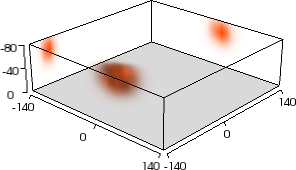
\includegraphics[width=4.5cm]{plots/vis_gaussian}\label{fig:SS-G}}%
    \subfigure[Single source 
    dispersion]{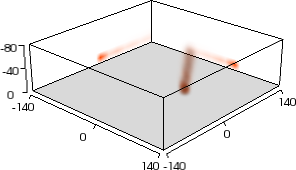
\includegraphics[width=4.5cm]{plots/vis_dispersion}\label{fig:SS-D}}%
    \subfigure[Multiple source 
    dispersion]{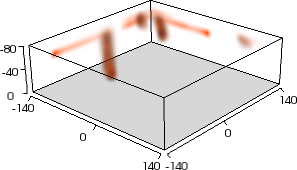
\includegraphics[width=4.5cm]{plots/vis_multi_dispersion}\label{fig:MS-D}}
    \caption[Visualizations of plume dispersions.]{Visualization of different 
        plume dispersions. The rear boundaries of the volume show 
        two-dimensional projections of concentration maxima in the respective 
        directions. Axes scale is in meters.}
\end{figure}

A Gaussian dispersion (D) as shown in Figure~\ref{fig:SS-D} is obtained when 
considering a constant wind parallel to the ground with velocity $u$ at 
\SI{6}{\meter} above the ground. The plume will be dispersed and form 
a cone-like distribution along the wind direction.  Making a few more 
assumptions (constant $Q$, steady-state, isotropic diffusion, no ground 
penetration, and neglegible variation in topography) the analytic expression
\begin{multline}
    c(\vc x') = \frac{Q}{2\uppi ua\del{x'_1 - s'_1}^b} 
    \exp\!\del{-\frac{\del{x'_2 - s'_2}^2}{2a\del{x'_1 - s'_1}^b}} \\ 
    \sbr{\exp\!\del{-\frac{\del{x'_3 - s'_3}^2}{2a\del{x'_1 - s'_1}^b}} 
        + \exp\!\del{\frac{\del{x'_3 + s'_3}^2}{2a\del{x'_1 - s'_1}^b}}}
\end{multline}
can be derived for the concentration \parencite{Stockie:2011fd}. Note that the 
coordinates $\vc x'$ and $\vc s'$ are expressed in the wind frame of reference. 
The wind speed is set to $u = \SI{3}{\meter\per\second}$ and the diffusion 
parameters to $a = \SI{0.33}{\meter\tothe{2 - \mathit{b}}}$ and $b = 0.86$.  The 
emission rate $Q$ is randomly and uniformly distributed chosen from the interval 
\SIrange{0.1}{2.5}{\gram\per\second}.

Sensor noise (SN) of the plume sensor is assumed to be additive and distributed 
according to $\mathcal{N}(0, \sigma\ped{noise}^2)$. In the noise free (NF) 
scenarios no noise was added to the measurements. The standard deviation 
$\sigma\ped{noise}$ was set to $10^{-4}$ in the scenarios including noise. The 
QRSim default scenarios set it to $10^{-2}$. But given the low default plume 
concentration this would require roughly averaging of 1600 samples from one 
single location to reduce the magnitude of the noise to the same level as the 
plume concentration values (see Appendix~\ref{sec:decnoise}). Hence, the default 
scenario is not solvable in a feasible amount of simulation time.

The overall concentration $c(\vc x)$ for $n$ sources like in 
Figure~\ref{fig:MS-D} is obtained by summing the individual contributions 
$c_i(\vc x)$ for each source:
\begin{equation}
    c(\vc x) = \sum_{i = 1}^n c_i(\vc x)
\end{equation}
In the scenarios with multiple sources (MS) $n$ is chosen uniformly out of the 
range from \numrange{1}{5}. With a single source it is fixed to $n = 1$. In both 
cases the source locations will be randomly chosen from a uniform distribution 
over the simulated volume.

The starting locations of the UAVs are also chosen randomly and uniformly in the 
simulated area, but the height is initially set to a starting height of $x_3 
= \SI{-10}{\meter}$. Either a single UAV (SV) or three UAVs (MV) were used.

This gives a number of possible scenarios from which I focussed on the following 
in this work:
\begin{itemize}
    \item In Chapter~\ref{sec:cmputility} I discuss the noise free, single 
        vehicles scenarios G-NF-SS-SV, D-NF-SS-SV, and D-NF-MS-SV\@. The first 
        is equivalent to the scenario 3A in \textcite{denardi2013rn}.
    \item In chapter TODO I consider the dispersion scenarios with noise 
        D-SN-SS-SV and D-SN-MS-SV\@. Except for the amount of noise these 
        correspond to scenario 3B and 3C in \textcite{denardi2013rn}.
    \item Finally, I will take a look at the usage of multiple vehicles with the 
        scenario D-SN-MS-MV corresponding to scenario 3D in 
        \textcite{denardi2013rn}.
\end{itemize}


\chapter{Gaussian Processes}
A vast number of regression methods has been proposed in the machine learning 
literature. In this work I use Gaussian Processes as these have been 
successfully used in a number of studies related to spatial and environmental 
monitoring including the modelling of gas distributions 
\parencite[e.g.][]{Stranders:2008wl, Marchant:2012wb, Stachniss:2008vz}.  
Gaussian Processes exhibit a number of desirable features. They are 
non-parametric, non-linear and therefore do not require any assumptions about 
the underlying functions or limitations of the search space.  Also, they provide 
one with an estimate of the predictive uncertainties which can be used for 
a natural exploration-exploitation trade-off.

In the remainder of the chapter I will discuss the essentials of Gaussian 
Process regression. A more thorough introduction can be found in 
\textcite{Rasmussen:2006vz}.

Let $\mathcal{D} = \{(\vc{x}_i, y_i) | i = 1, \dots, N\}$ a set of training data 
with inputs $\vc x$ and outputs $y = f(\vc x) + \eta$ with additive noise $\eta 
\sim \mathcal{N}(0, \sigma\ped{n}^2)$. We want to learn the function $f(\vc x)$ 
from this training data.

A Gaussian Process
\begin{equation}
    f(\vc x) \sim \mathcal{GP}(m(\vc x), k(\vc x, \vc x'))
\end{equation}
imposes a multivariate Gaussian distribution on the space of functions $f(\vc 
x)$. It is completely specified by the mean function $m(\vc x)$ and covariance 
function $k(\vc x, \vc x')$. Usually, though not necessary, the mean function is 
taken to be zero. In most scenarios the choice of the covariance function is 
much more interesting as it controls features like smoothness of the predicted 
underlying function. I will discuss this topic regarding the modelling problem 
on hand in Section~\ref{sec:covfn}.

We can now formulate the joint Gaussian prior distribution of the observed 
training targets and the predicted values $\vc f_*$ at unseen locations $X_*$ 
(assuming $m(\vc x) = 0$):
\begin{equation}
    \left[ \begin{array}{c}\vc y \\ \vc f_* \end{array} \right]
    \sim \mathcal{N}\left(\vc 0,
        \left[ \begin{array}{cc}
            K(X, X) + \sigma\ped{n}^2 \mat I & K(X, X_*) \\ K(X_*, X) & K(X_*, 
            X_*)
        \end{array} \right]
    \right)
\end{equation}
Here $K(X, X')$ are matrices with the elements $(i, j)$ being the covariances 
$k(\vc x_i, \vc x'_j)$ evaluated for all pairs $\vc x_i \in X$ and $\vc x'_j \in 
X'$. In the following I will use $\tilde{\mat K} = K(X, X) + \sigma\ped{n}^2 
\mat I$ as a shorter notation. By conditioning on the observations one obtains 
the predictive distribution for $\vc f_*$ as
\begin{align}
    \vc f_* | X, \vc y, X_* &\sim \mathcal{N}(\bar{\vc f_*}, \cov(\vc 
    f_*))\text{, with}\\
    \bar{\vc f_*} &= \mu(X_*) = K(X_*, X)\tilde{\mat K}^{-1} \vc y\text{,} \\
    \cov(\vc f_*) &= K(X_*, X_*) - K(X_*, X)\tilde{\mat K}^{-1}K(X, X_*) 
    \\
    \sigma^2(X_*) &= \diag(\cov(\vc f_*)) \text{.}
\end{align}
See Figure~\ref{fig:ex-gp-main} for a visualization of an example Gaussian 
process.

\begin{figure}
    \centering
    \subfigure[]{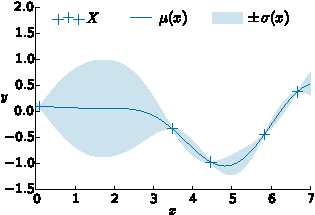
\includegraphics{plots/gp}\label{fig:ex-gp}}%
    \subfigure[]{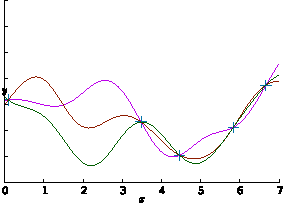
\includegraphics{plots/gp_sample}\label{fig:ex-gp-sample}}
    \caption[Gaussian process example]{Example of a one-dimensional Gaussian 
        process (using the squared exponential covariance function with 
        a length-scale of 1, $\sigma\ped{n}^2 = 0$) conditioned on five training 
        points: \subref{fig:ex-gp} shows the mean $\bar{\vc f_*}$ and predictive 
        standard deviation $\sigma(X_*)$; \subref{fig:ex-gp-sample} shows three 
        functions sampled from the process.}\label{fig:ex-gp-main}
\end{figure}

Even though, $K$ is a symmetric, positive-definite matrix it can be 
ill-conditioned.\footnote{The condition $\kappa(A)$ of a matrix $A$ is defined 
    as $\kappa(\mat A) = \|\mat A\| \|\mat A^{-1}\|$. Using the $L_2$-norm this 
    corresponds to $\kappa(\mat A) = \frac{\lambda_1}{\lambda_n}$,
    the ratio of the largest eigenvalue $\lambda_1$ and the smallest one
    $\lambda_n$. If the condition number $\kappa(\mat A)$ is too large, the 
    matrix is near-singular and ill-conditioned.} This happens especially for 
close-by input data points as they occur in a sequential scenario like the plume 
modelling here.

There are two commonly implemented approaches to counteract the problem of 
ill-conditioning \parencite[cp.]{Sacks:1989cv, Neal:1997tj, Booker:1999wz, 
    Gramacy:2008es}. Firstly, instead of using a general matrix inversion 
algorithm one can utilize the symmetry and positive-definiteness of 
$\tilde{\mat{K}}$ by doing a Cholesky decomposition. That yields a lower, 
triangular matrix $L$ satisfying $\tilde{\mat K} = \mat L\mat L\Tr$. The inverse 
can the be calculated as $\tilde{\mat K}^{-1} = (\mat L^{-1})\Tr \mat L^{-1}$.  
Secondly, a well conditioned $\tilde{\mat K}$ can be ensured by adding a nugget 
$g > 0$ (also known as jitter) to the diagonal of the covariance matrix. This 
will increase all eigenvalues by the same value and thus improve the condition.  
The addition of a nugget can also be seen as increasing the noise variance 
$\sigma\ped{n}^2$ and thus allowing the Gaussian Process to match the target 
less precisely and to become smoother.

\section{Online Updates}
A naive implementation requires a $O(N^3)$ matrix inversion whenever new data 
points are added to the Gaussian Process with $N$ being the total number of data 
points collected so far. However, it is possible to do online updates with $n 
< N$ new data points where only a $n \times n$ matrix has to be inverted. This 
reduces the complexity of the matrix inversion to $O(n^3)$ and the overall 
complexity including the necessary matrix multiplications to $O(n\,{[\max\{n, 
    N - n\}]}^2)$.

Let us denote the set of inputs already trained on with $X$ and the set of 
inputs to add as $X'$. The block covariance matrix after adding these new inputs 
will be
\begin{equation} \label{eqn:tilde_K_prime}
    \tilde{\mat K}' = \left[ \begin{array}{cc}
            \tilde{\mat K} & K(X, X') \\ K(X', X) & K(X', X') 
            + \sigma\ped{n}^2\mat I
        \end{array}
    \right]\text{.}
\end{equation}
The Cholesky factorization can also be written with block matrices
\begin{equation}
    \tilde{\mat K}' = \mat L \mat L\Tr = \left[
        \begin{array}{cc}
            \mat A & \mat 0 \\ \mat B & \mat C
        \end{array}
    \right] \left[
        \begin{array}{cc}
            \mat A\Tr & \mat B\Tr \\ \mat 0 & \mat C\Tr
        \end{array}
    \right] = \left[
        \begin{array}{cc}
            \mat A \mat A\Tr & \mat A \mat B\Tr \\ \mat B \mat A\Tr & \mat B \mat 
            B\Tr + \mat C \mat C\Tr
        \end{array}
    \right]
\end{equation}
and comparison with equation~(\ref{eqn:tilde_K_prime}) gives the following 
relations:
FIXME\@: the L is used for two different sized matrices!
\begin{align}
    \mat A &= \mat L \\
    \mat B &= K(X', X) \del{\mat L\Tr}^{-1} \\
    \mat C \mat C\Tr &= K(X', X') + \sigma\ped{n}^2\mat I - K(X', 
    X)\tilde{\mat{K}}^{-1}K(X, X')
\end{align}
As $\mat C \mat C\Tr$ is symmetric, positive-definite it is possible to obtain 
$\mat C$ by a Cholesky decomposition.
With the inverse of a block matrix \parencite[45]{Petersen:2008wc} we obtain the 
following relation for the inverse of the updated Cholesky factor:
\begin{equation}
    \mat L' = \left[
        \begin{array}{cc}
            \mat L^{-1} & \mat 0 \\ -\mat C^{-1} K(X', X)\tilde{\mat K}^{-1} 
            & \mat C^{-1}
        \end{array}
    \right]
\end{equation}

\section{Sparse Approximations}

\section{Covariance Functions}\label{sec:covfn}
The choice of the covariance function determines the assumptions about the 
functions learned with a Gaussian process. Hence, it is quite important. In this 
chapter I will discuss some widely used covariance functions and considerations 
to take into account. A more thorough discussion including further covariance 
functions is to be found in \textcite[Chapter 4]{Rasmussen:2006vz} on which this 
section is based.

A valid covariance function $k(\vc x, \vc x')$ has to be semi-positive definite 
kernel \parencite{Cressie:1993uu} satisfying
\begin{equation}
    \int f(\vc x) k(\vc x, \vc x') f(\vc x') \dif \mu(\vc x) \dif \mu(\vc x') 
    \geq 0
\end{equation}
with $f \in L_2(\mathcal{X}, \mu)$. This ensures that the kernel's Gram matrix 
for a set of inputs $\cbr{x_i | i = 1, \dots, n}$ with entries $\mat K_{ij} 
= k(\vc x_i, \vc x_j)$ is also semi-positive definite and therefore a valid, 
invertible covariance matrix.

The choice of covariance function determines the smoothness of the Gaussian 
process. This is formalized in the notion of how many times it is \newterm{mean 
    square (MS) differentiable}. A process $f(\vc x)$ is differentiable if the
mean square limit denoted by $\mslim$ exists in the mean square derivative given 
by
\begin{equation}
    \dpd{f(\vc x)}{x_i} = \mslim_{h \rightarrow 0} \frac{f(\vc x + h\vcc e_i) 
    - f(\vc x)}{h}
\end{equation}
for the $i$-th direction with the unit vector $\vcc e_i$.

%defined in \textcite[81]{Rasmussen:2006vz} in the following way: ``Let $x_1, 
%x_2, \dots$ be a sequence of points and $x_*$ be a fixed point in $\mathbb{R}^D$ 
%such that $\abs{x_k - x_*} \rightarrow 0$ as $k \rightarrow \infty$. Then 
%a process $f(x)$ is continuous in mean square at $x_*$ if 
%$\mathbb{E}[\abs[0]{f(x_k) - f(x_*)}^2] \rightarrow 0$ as $k \rightarrow 
%\infty$. If this holds for all $x_* \in A$ where $A$ is a subset of 
%$\mathbb{R}^D$ then $f(x)$ is said to be continuous in mean square (MS) over 
%$A$.''

\subsection{Stationary Covariance Functions}
A kernel which is only a function of $\vc x - \vc x'$ is called 
\newterm{stationary} and is invariant to translations. Furthermore, it is 
\newterm{isotropic} if it is a radial basis function (RBF) $k(r)$ with $r 
= \abs{\vc x - \vc x'}$.  An isotropic kernel is invariant to all rigid motions.

For stationary kernels the smoothness properties of the resulting Gaussian 
process can be easily obtained: It is $k$-times differentiable if at $\vc 
x = \vc 0$ the $2k$-th order partial derivatives $\partial^{2k} k(\vc x) 
/ \partial x_{i_1}^2 \dots \partial x_{i_k}^2$ exist and are finite. Thus, the 
process smoothness is essentially determined by the kernel properties around 
$\vc 0$.

A common default choice is the \newterm{squared exponential} (SE) kernel defined 
as
\begin{equation}
    k\ped{SE}(r) = \sigma_k^2 \exp\del{-\frac{r^2}{-2\ell^2}}
\end{equation}
with the desired process variance $\sigma_k^2$ and length-scale $\ell$. It 
produces infinitely MS differentiable Gaussian processes. This can, actually, be 
too smooth in many applications.

The Mat\'ern class of covariance functions allows to control the smoothness with 
a parameter $\nu$. Using the modified Bessel function $K_{\nu}$ it is given by
\begin{equation}
    k_{\nu}(r) = \sigma_k^2 \frac{2^{1-\nu}}{\Gamma(\nu)} 
    \del{\frac{r\sqrt{2\nu}}{\ell}}^{\nu} K_{\nu} 
    \del{\frac{r\sqrt{2\nu}}{\ell}}
\end{equation}
The resulting Gaussian process will be $k$ times MS differentiable for $k 
< \nu$. The parameter $\ell$ denotes again the characteristic length-scale.

Typically, only the kernels with $2\nu \in \cbr{1, 2, 3}$ are used.  Usually the 
(noisy) data allows not to differentiate which kernel to use for larger $\nu$.  
Half-integer values are used as the kernel function will become quite simple:
\begin{align}
    k_{5/2}(r) &= \sigma_k^2 \del{1 + \frac{r\sqrt{5}}{\ell} 
        + \frac{5r^2}{3\ell^2}} \exp\del{-\frac{r\sqrt{5}}{\ell}} \\
    k_{3/2}(r) &= \sigma_k^2 \del{1 + \frac{r\sqrt{3}}{\ell}} 
    \exp\del{-\frac{r\sqrt{3}}{\ell}} \\
    k_{1/2}(r) &= k_{\exp}(r) = \sigma_k^2 \exp\del{-\frac{r}{\ell}}
\end{align}
From these kernel functions $k_{\nu=1/2}(r)$ is also known as the 
\newterm{exponential kernel}. Furthermore, note that for $\nu \rightarrow 
\infty$ the squared exponential kernel is recovered. A plot of the covariance 
functions can be found in Figure~\ref{fig:kernels}.

\begin{figure}
    \centering
    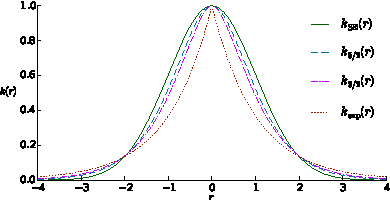
\includegraphics{plots/kernels}
    \caption[Covariance functions]{Plot of stationary covariance functions with 
        $\sigma_k^2 = 1, \ell = 1$.}\label{fig:kernels}
\end{figure}

TODO include MS continuity?

\subsection{Non-stationary Covariance Functions}
Many phenomena, including the concentrations of gas plumes, are not stationary.  
Already a Gaussian density function exhibits different optimal length-scales 
(see Figure~\ref{fig:gp-lengthscale}).  With a long length-scale the predicted 
mean can considerably deviate from the target function as shown for positive $x$ 
in the figure. With a short length-scale a quite good fit is obtained. However, 
the predictive variance along the tail towards negative $x$ is overestimated as 
the actual rate of change in this area is quite low.

\begin{figure}
    \centering
    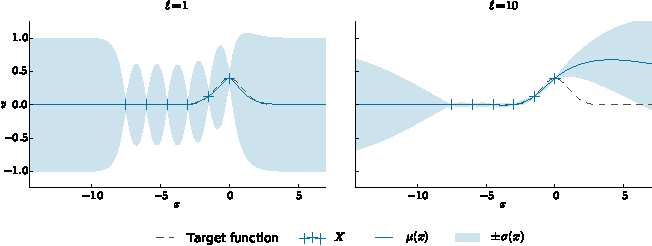
\includegraphics{plots/gp-lengthscale}
    \caption[Length-scale influence]{Influence of the kernel length-scale on the 
        Gaussian process. In both plots the Mat\'ern kernel with $\nu = 3/2$ was 
        used. On the left a short length-scale of $\ell = 1$ was used, whereas 
        a longer length-scale of $\ell = 10$ was used on the right.
    }\label{fig:gp-lengthscale}
\end{figure}

Non-stationary covariance functions can alleviate this problem. Moreover, they 
allow to model discontinuities at specific places. However, the usage of 
non-stationary covariance functions for the given plume modelling problem is far 
from straight forward and might need more prior knowledge than one is willing to 
assume (in simulations) or effectively has.  One would probably have to use 
different kernels depending on the scenario (wind/no wind, number of sources) 
and these would have to be parameterized with the source locations. Otherwise 
the non-stationarity of the kernel could not relate to the actual 
non-stationarity of the plume.

Methods for selecting such parameters will be discussed in the next section.  
Unfortunately, the cost of these methods grows with the number of parameters 
which for non-stationary kernels will be larger. Matters are complicated even 
more as it is usually desirable to have a differentiable kernel to be able to 
use gradient-based optimizers. In an active learning scenario, moreover, there 
is a limited amount of data in the beginning making the correct estimation of 
parameters like the source position virtually impossible.

TODO read and maybe include non-stationary papers
TODO non-stationary not agnostic to structure.

\section{Hyper-parameter Selection}
Though Gaussian processes are non-parametric, the choice of covariance function 
will introduce hyper-parameters $\vc \theta$ like the length-scale which have to 
be set.  In the following I will discuss three methods for doing so.

With the \newterm{test set method} all data available $\mathcal{D}$ will be 
split into two sets $\mathcal{D}_0$ and $\mathcal{D}_*$. The first one 
$\mathcal{D}_0$ is used to train Gaussian processes with different covariance 
functions and hyper-parameters. For each model the generalization error 
$E\ped{G}$ over the test set $\mathcal{D}_*$ will be evaluated and one choses 
the parameters with the minimal generalization error. The error measure can be 
chosen freely, with the root mean square error being a typical choice (see also 
section TODO).

If the amount of data available is low, it is common to use \newterm{$k$-fold 
    cross validation} where $\mathcal{D}$ is split into $k$ disjoint subsets 
$\mathcal{D}_i$ of equal size and the generalization error will be calculated 
from $k$ models using the respective $\mathcal{D}_i$ as test set and the other 
sets as training data.

The third possibility is to find $\argmax_{\vc \theta} p(\vc\theta | \vc y, \mat 
X, \mathcal{H}_i)$, wherein
\begin{equation}
    p(\vc\theta | \vc y, \mat X, \mathcal{H}_i) = \frac{p(\vc y | \mat X, 
        \vc\theta, \mathcal{H}_i) p(\vc\theta | \mathcal{H}_i)}{p(\vc y | \mat 
        X, \mathcal{H}_i)}
\end{equation}
with marginal likelihood $p(\vc y | \mat X, \vc\theta, \mathcal{H}_i)$, prior 
$p(\vc\theta | \mathcal{H}_i)$, normalization factor $p(\vc y | \mat X, 
\mathcal{H}_i)$, and a set of possible model structures $\mathcal{H}_i$. The 
normalization factor can be difficult to estimate 
\parencite[109]{Rasmussen:2006vz}. For that reason often, even thought it can 
more easily lead to overfitting, only the marginal likelihood is optimized which 
is known as type~II maximum likelihood. For a Gaussian process with $n$ training 
samples it is given by
\begin{equation}
    \log p(\vc y | \mat X, \vc\theta) = -\frac{1}{2}\del{\vc y\Tr 
        \tilde{\mat{K}}^{-1} \vc y + \log \det \tilde{\mat K} + n \log 2\uppi} 
    \text{.}
\end{equation}
The three summands can be interpreted as the quality of the data fit $\vc y\Tr 
\tilde{\mat K}^{-1} \vc y$, model complexity $\log \det \tilde{\mat K}$, and 
a normalization term $n \log 2\uppi$. Hence, the optimization of the marginal 
likelihood includes an automatic trade-off of model complexity and data fit.

Optimizing the marginal likelihood has the advantage in comparison to the test 
set method that a gradient based optimizer can be used. The partial derivatives 
of the likelihood are given by
\begin{equation}
    \dpd{}{\theta_j} \log p(\vc y | \mat X, \vc\theta) = \frac{1}{2} 
    \del{\del{\tilde{\mat K}^{-1}\vc y \vc y\Tr \tilde{\mat K}^{-1} 
            - \tilde{\mat{K}}^{-1}} \dpd{\tilde{\mat K}}{\theta_j}} \text{.}
\end{equation}
However, all method require a complete retraining of the Gaussian process as for 
each update of the hyper-parameters $\tilde{\mat K}^{-1}$ has to be newly 
calculated. Thus, in an online setting it is far more efficient to keep the 
hyper-parameters fixed or only update them occasionally.

TODO Gaussian Process Mixtures? Efficiency in case of parallel calculation?
How is the selection happening? Error or likelihood?

\section{Active Learning}
TODO scaling is not correct

A setting in which a learning algorithm can freely choose the next training 
input is called \newterm{active learning}. A general introduction in the topic 
is provided by \textcite{Settles:2009vo}. Here, I will focus on how to realize 
active learning in the context of Gaussian processes.

In general, one defines a \newterm{utility} or \newterm{acquisition} function 
$u(\vc x)$ indicating the expected benefit for choosing $\vc x$ as next training 
sample. Hence, the optimal choice is $\argmax_{\vc x} u(\vc x)$. Equivalently, 
it is possible to use the negative of a loss function $u(\vc x) = - \lambda(\vc 
x)$.

The choice of $u(\vc x)$ influences the exploration-exploitation trade-off and 
on which areas of the input space the learning will be focussed. In the 
estimation of a plume distribution samples should be acquired mostly at places 
with high concentrations, but once such an area is well estimated further 
exploration should follow to possibly find further sources.

\Textcite{Marchant:2012wb} proposed the \newterm{distance-based upper confidence 
    bound} (DUCB) for a similar scenario of environmental monitoring where ozone 
concentrations over US territory were to be measured:
\begin{equation}
    u\ped{DUCB}(\vc x) = \mu(\vc x) + \kappa \cdot \sigma^2(\vc x) + \gamma 
    \cdot d(\vc x, \vc x')
\end{equation}
The mean prediction $\mu(\vc x)$ and the predictive variance $\sigma^2(\vc x)$ 
are obtained directly from the Gaussian process, $d(\vc x, \vc x')$ denotes the 
Euclidean distance of $\vc x$ to the last sample location $\vc x'$. The 
parameter $\kappa$ controls the exploration-exploitation balance. Higher values 
give more importance to decreasing the predictive variance and lead to more 
exploration. The parameter $\gamma \leq 0$ adjusts the distance penalty.  
Favoring location near to the current UAV position might decrease the distance 
travelled and save energy as well as time.

Though, the scenario above appears to be quite similar to the problem at hand 
one should note a certain difference. The ozone concentration is a quite smooth 
distribution as \textcite{Marchant:2012wb} used the squared exponential 
covariance function to obtain reasonable results. In opposite to that, the 
spatial distribution of a gas plume is much more localized \parencite[][this was 
also noted by]{Stachniss:2008vz}. Thus, I propose \newterm{plume distance-based 
    upper confidence bound} (PDUCB) acquisition function inspired by DUCB, but 
adjusted:
\begin{equation}
    u\ped{PDUCB}(\vc x) = \del{1 - a} \cdot \ln\del{\mu_+(\vc x) + \varepsilon} 
    + a \cdot \ln \varepsilon + \kappa \cdot \sigma^2(\vc x) + \gamma \cdot 
    d^2(\vc x, \vc x')
\end{equation}
with
\begin{align}
    a &= \e^{-\mu_+(\vc x) / \varepsilon} \\
    \mu_+(\vc x) &= \max\cbr{0, \mu(\vc x)}
\end{align}

Using the logarithm of the prediction mean makes this utility function sensitive 
for small concentrations which can hint towards areas with higher concentration.  
Being sensitive to the same absolute change for high concentrations is not as 
important. As the concentration might be equal to zero strict positiveness has 
to be explicitly ensured by a small $\varepsilon > 0$. Also, strict positiveness 
of the predictive mean has to be ensured. It is desirable to have differentiable 
acquisition functions to be able to used gradient based optimizers. However, due 
to the logarithm the function would not be differentiable for $\mu(\vc x) 
\rightarrow 0$. Thus, it is weighted with $(1 - a)$ and faded out to $\ln 
\varepsilon$ to restore differentiability (proof in appendix TODO).

A further change in PDUCB compared to DUCB is the squaring of the distance which 
will reduce the penalty around $\vc x'$ (while increasing it further away).  
This should be advantageous as the unsquared distance function tends to force 
$\vc x$ much closer to $\vc x'$, but the next sample though it should be near to 
$\vc x'$ should not be too close to $\vc x'$.  Otherwise, not much new 
information would be gained.

Apart from some explicit values, \textcite{Marchant:2012wb} do not discuss how 
to choose the parameters $\kappa$ and $\gamma$. Nevertheless, some observations 
can be made for both DUCB and PDUCB\@. Firstly, one should choose $\kappa \cdot 
\max \sigma^2(\vc x) > \max \mu(\vc x)$. Otherwise, one can get stuck in a local 
maximum as the mean prediction term might get larger than the predictive 
variance anywhere in the input space. Even though, it can be a good strategy to 
exploit maxima first exploration should continue once the distribution around 
the maximum is accurately known. A too small $\kappa$ is also problematic as it 
prevents any exploitation. Secondly, $\abs{\gamma}$ should not be too large or 
the distance penalty would dominate and also lead to one getting stuck in one 
position $\vc x = \vc x'$. Thirdly, $\varepsilon$ influences the sensitivity for 
low concentrations and should therefore be small, but large enough too prevent 
numerical problems in the evaluation of the logarithm. A value of $\varepsilon 
= 10^{-30}$ seems to work well (see section TODO).

Typically, one knows the spatial dimensions of the input space which allows to 
estimate a reasonable $\gamma$ in relation to $\kappa$ as the maximual 
predictive variance is given by $\sigma\ped{n} + \sigma\ped{k}$.  However, the 
maximal $\vc y$ determining $\max \mu(\vc x)$ which is important for the 
absolute values of $\gamma$ and $\kappa$ might not be known in advance.  Thus, 
it would be helpful to set these parameters automatically from $\vc y$, the data 
seen so far.  This can be done by setting
\begin{align}
    \kappa &= s(\vc y) \cdot \kappa' \\
    \gamma &= s(\vc y) \cdot \gamma'
\end{align}
with a scaling factor $s(\vc y)$ defined for the respective acquisition 
functions as
\begin{align}
    s\ped{DUCB}(\vc y) &= \max \vc y \\
    s\ped{PDUCB}(\vc y) &= \ln(\max \vc y + \varepsilon) - \ln \varepsilon 
    \text{.}
\end{align}
The new parameters $\kappa'$ and $\gamma'$ can then be set independent of the 
actual values of $\vc y$.

A third potential acquisition function, also balancing exploration and 
exploitation, can be derived from the work by \textcite{Osborne:2009tn}. They 
introduce a Bayesian approach for global optimization. Adopting their approach 
for a one-step look-ahead one first defines a loss function equal to the 
negative of the newly observed maximum
\begin{equation}
    \lambda\ped{GO} (y_*) = \left\{ \begin{array}{ll}-y_* & y_* > \eta \\ -\eta 
            & y_* \leq \eta \end{array} \right.
\end{equation}
with $\eta = \max \vc y$. From this the expected loss can be determined as
\begin{equation}\begin{split}
    \varLambda\ped{GO}(\vc x) &= \int \lambda\ped{GO}(y_*) p(y_* | \vc x, X, \vc 
    y) \dif y_* \\
    &= -\eta - \del{\mu(\vc x) - \eta} \varPhi\!\del{\eta; \mu(\vc x), 
        \sigma^2(\vc x)} - \sigma^2(\vc x) N\!\del{\eta; \mu(\vc x), 
        \sigma^2(\vc x)}
    \text{.}
\end{split}\end{equation}
In this equation $N(x; \mu, \sigma^2)$ and $\varPhi(x; \mu, \sigma^2)$ are the 
Gaussian probability density and respectively the Gaussian cummulutative 
distribution function with mean $\mu$ and variance $\sigma^2$. Adding a distance 
penalty term to the negative of $\varLambda\ped{GO}(\vc x)$ gives the final 
utility function
\begin{equation}\begin{split}
    u\ped{GO}(\vc x) &= -\varLambda\ped{GO}(\vc x) + \gamma' \cdot d^2(\vc x, 
    \vc x') \\
    &= \eta + \del{\mu(\vc x) - \eta} \varPhi\!\del{\eta; \mu(\vc x), 
        \sigma^2(\vc x)} + \sigma^2(\vc x) N\!\del{\eta; \mu(\vc x), 
        \sigma^2(\vc x)} + \gamma' \cdot d^2(\vc x, \vc x')
    \text{.}
\end{split}\end{equation}
TODO include multi-step look-ahead? process mixtures?

\begin{figure}
    \centering
    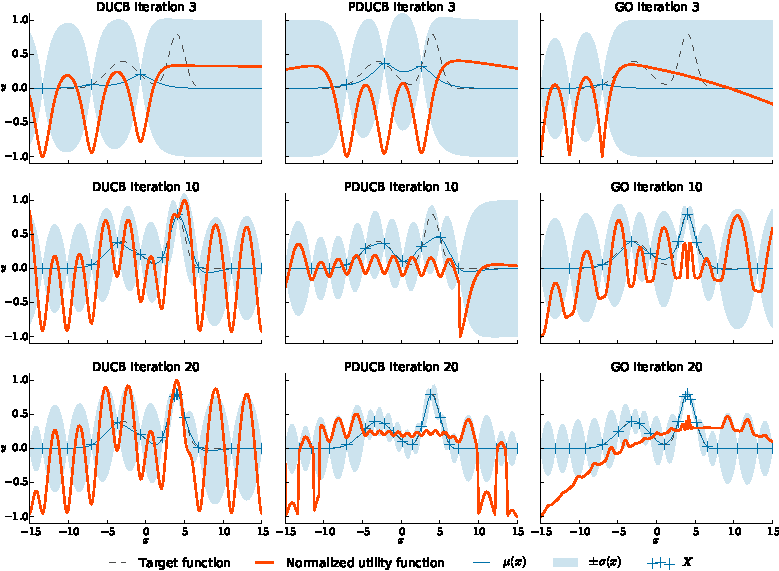
\includegraphics{plots/acqfns}
    \caption{Visualization of acquisition functions. The columns of the plot 
        matrix correspond to the three different acquisition functions (DUCB, 
        PDUCB, GO) and the rows show the state after 3, 10, and 20 iterations.  
        The parameters used for these plots were $\kappa' = 1.25$, $\gamma' 
        = -0.0002$, $\varepsilon = 10^{-30}$, $s\ped{DUCB} = 1$, and 
        $s\ped{PDUCB} = 70$. The inital sample was always chosen at $x_0 
        = -7$.}\label{fig:acqfns}
\end{figure}
In Figure~\ref{fig:acqfns} a grapihcal comparison of the proposed utility 
functions is given for a one-dimensional example. It can be seen that DUCB 
heavily focusses on the function maximum without much exploration in other 
areas. The GO acquisition function also acquires more samples around the 
maximum, but reduces the uncertainty more equally over the domain. In comparison 
to these to functions PDUCB seems also to focus around the maxima, but with 
a wider exploration around those. In Chapter TODO I will more closely look on 
how well these functions work to estimate a plume dispersion with different 
parameter choices.

\subsection{Multiple UAVs}

\subsection{Bootstrapping}
As long as not a minimal concentration has been measured all of the proposed 
acquisition functions do not have a unique maximum. Though one could choose one 
of the many maxima randomly, this might take a long time until the plume gets 
discovered. Hence, it is best to employ a more systematic search strategy in the 
beginning.

Here, three variations have been used. First, surrounding the area in a medium 
height. Without noise this should be sufficient to obtain enough information for 
a successful usage of the discussed acquisition functions.

Considering noise a second strategy is needed as measurements of low 
concentrations are not reliably anymore. This strategy consists of surrounding 
the area at different heights until the criterion that a plume as been found is 
fulfilled. The criterion was that the maximum of all concentration measurements 
$C$ for one surrounding has to be larger than $5\sigma(C)$ with $\sigma(C)$ 
being the standard deviation of $C$.

This second strategy may also take a long time until a plume has been found, but 
should be faster than only random exploration. If the wind direction is known 
(which is not the case in the standard QRSim scenarios), a third strategy can be 
used. It improves the second strategy by not doing complete surrounds of the 
area, but only along the two area edges which are ``hit'' by the wind as those 
the only two were the plume might be detected.

These bootstrapping strategies can be easily extended to multiple UAVs by 
assigning different heights to each one.

TODO only part of samples are used to train GP

\chapter{Error Measures}
To be able to compare different statistical models some kind of performance 
measure, usually in the form of an error measure, is needed. In the plume 
modelling task one is interested in the deviation of the predicted 
concentrations $\mu(\vc x)$ from the true ones $c(\vc x)$. When using the $L^2$ 
norm and integrating over the complete task volume $V$ the root mean integrated 
square error (RMISE)
\begin{equation}
    E\ped{RMISE} = \sqrt{\frac{1}{v} \int_V \del{c(\vc x) - \mu(\vc x)}^2 
        \dif\vc x}
\end{equation}
with
\begin{equation}
    v = \int_V \dif\vc x
\end{equation}
is obtained. However, it can be assumed that accurate predictions are more 
important where the concentrations is actually high 
\parencite[c.p.][]{Marchant:2012wb}. Thus, it might be beneficial to introduce 
a weighting factor $w(\vc x)$ to
\begin{equation}
    E\ped{WRMISE} = \sqrt{\frac{1}{v} \int_V \del{c(\vc x) - \mu(\vc x)}^2 w(\vc 
        x) \dif\vc x} \text{,}
\end{equation}
the weighted root mean integrated square error (WRMISE), with
\begin{equation}
    w(\vc x) = \frac{c(\vc x) - \min c(\vc x')}{\max c(\vc x') - \min c(\vc x')} 
    \text{.}
\end{equation}
Note that in areas with an almost or even exactly zero concentration the WISE 
will always be close to zero and thus allowing the model to make highly 
inaccurate predictions. Therefore, the WISE should not be used as sole measure 
in plume modelling. Using both errors it is possible to ensure an good overall 
fit of the prediction without large inaccuracies and to compare which model has 
the better fit in the interesting areas.

Unfortunately, the ISE and WISE cannot easily be calculated analytically and one 
has to restrain to approximating the integral from a set $\{\vc x_i | i = 1, 
\dots, n\}$ of finite size $n$. If the $x_i$ are distributed according to the 
probability density function $p(\vc x)$, the discrete approximation has the form
\begin{align}
    \hat E\ped{RMISE} &= \sqrt{\frac{1}{vZ} \sum_{i=1}^n \frac{\del{c(\vc x_i) 
                - \mu(\vc x_i)}^2}{p(\vc x_i)}} \\
    \hat E\ped{WRMISE} &= \sqrt{\frac{1}{vZ} \sum_{i=1}^n \frac{\del{c(\vc x_i) 
                - \mu(\vc x_i)}^2 w(\vc x_i)}{p(\vc x_i)}} \text{.}
\end{align}
The normalization constant $Z$ is given by
\begin{equation}
    Z = \sum_{i=1}^n \frac{1}{p(\vc x_i)} \text{.}
\end{equation}

The probability density $p(\vc x)$ can be estimated using Gaussian kernel 
density estimation (KDE). (TODO ref) There exist different methods to determine 
the bandwidth parameter of the KDE\@. I used in this work Scott's Rule (TODO 
ref).

\section{Selecting Samples for Error Approximation}
Up to now it is still open how to select the $x_i$ for approximating the error 
measures.  Using a regularly spaced grid is either likely to miss the important 
areas as the plume is quite localized or it is so fine grained that the 
evaluation of the error takes a long time. Also, sampling uniformly from the 
volume is likely to miss the interesting areas.  Thus, I used a slightly 
modified Metropolis-Hastings algorithm to concentrate samples in areas with 
a high concentration.

The standard Metropolis-Hastings (TODO ref) is used to sample from a probability 
distribution $P(\vc x)$ given only a function $f(\vc x)$ proportional to $P(\vc 
x)$. It starts at a random location $\vc x_1$.  Then in each iteration $i > 0$ 
a new candidate location $\vc x_*$ is picked from a symmetric\footnote{$Q(\vc 
    a | \vc b) = Q(\vc b | \vc a)$} proposal distribution and an acceptance 
ratio $r = f(\vc x_*) / f(\vc x_i)$ is calculated. The candidate $\vc x_*$ is 
accepted as $\vc x_{i + 1} = \vc x_*$ with probability $r$ ($r \geq 1$ 
automatically accepts). If it is rejected, $\vc x_{i + 1} = \vc x_i$ will be 
used.

To select the samples for the error approximation this algorithm can be used 
with the true concentrations $f(\vc x) = c(\vc x)$. For this purpose it is not 
necessary that the samples follow a specific probability distribution. That 
makes it possible to make a few adoptions for better results.

First of all, $\vc x_*$ gets always added to the set of samples independent of 
acceptance or rejection.  This makes each location unique (as long as the same 
location does not get proposed twice).  Having multiple instance of the same 
location within the samples would not increase the accuracy of the error 
approximation. Also, this leads to a few more samples towards the concentration 
tails where the concentration is already low but close to high concentrations.  
Thus, the approximation around the concentration slope can be expected to be 
better.

The second change concerns the initial location $\vc x_1$. Choosing at randomly 
might place it in an area with zero concentration which renders the acceptance 
ratio $r$ undefined. Hence, it is better base the initial location on the source 
locations. Unfortunately, given a plume dispersion (TODO ref eq) the plume 
concentration is undefined at the source location (TODO appendix). To circumvent 
this, the initial location $\vc x_1$ should be excluded from the samples.

In case of multiple sources it should be started from each source location and 
the resulting sets should be joined. The concentration between sources can be 
rather low making it unlikely to switch from one plume to another. Also, the 
Metropolis-Hastings algorithm is unlikely to sample in low concentration areas, 
especially in some distance to the plumes. Thus, a number of uniformly sampled 
locations should be added.

To ``smooth'' out the samples around the plumes even more one can use the 
samples of the Metropolis-Hastings algorithm as center of Gaussian distributions 
and draw a number of further samples from these.
TODO not completely correct, just take every n-th sample

TODO pics

\section{QRSim Reward}
The plume modelling scenario in \textcite{denardi2013rn} them self define 
a reward
\begin{equation}
    R = - \sum_{i = 1}^n \del{c(\vc x) - \mu(\vc x)}^2
\end{equation}
as a performance measure. This is essentially the negative of 
$\hat{E}\ped{RMISE}^2$ without normalization. Thus, with a non uniform sampling 
this reward will give a biased estimate attributing more importance to areas 
with more sample locations.

The set of $\vc x_i$ used to calculate the reward in QRSim consists ouf of two 
parts. One-fifth is sampled uniformly over the whole volume whereas the 
remaining samples are taken uniformly from the areas where the concentration 
exceeds the limit $c_{\min} = Q \cdot 10^{-3} \cdot 
\si{\second\per\meter\cubed}$.

The bias introduced by that towards the interesting regions is not necessarily 
bad. The same is done in the weighted root mean integrated square error.  
Unfortunately, the sampling strategy will not sample at the low side of 
a (steep) concentration boundary and will give an bad estimate of the reward 
around those boundaries. In contrast to that, the Metropolis-Hastings based 
sampling algorithm acquires also some samples low concentration area around 
a high concentration. Figure~\ref{fig:err-sampling} provides a comparison of 
both sampling strategies.

\begin{figure}
    \centering
    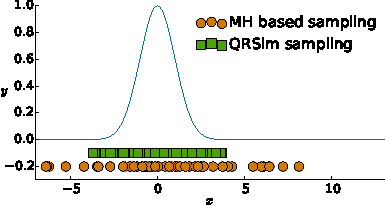
\includegraphics{plots/err-sampling}
    \caption[Comparison of error estimation sampling methods]{One-dimensional 
        comparison of the Metropolis-Hastings (MH) based sampling and the QRSim 
        sampling for error estimation. For both approaches 60 samples with 
        regard to the plotted Gaussian density were taken excluding the 
        uniformly distributed samples.  The $y$ position of the scatter marks 
        has no meaning in this plot. For this plot every fifth sample of the 
        Metropolis-Hastings algorithm was used.  A Gaussian was used as proposal 
        distribution with $\sigma = 2$.  The same distribution was used to 
        create five additional samples for each initial 
        one.}\label{fig:err-sampling}
\end{figure}

\chapter{Technical Details}
To implement the discussed algorithms in a functioning system some further 
details have to be taken in consideration. I will discuss these in this chapter 
after giving short general overview of the implementation.

\section{Implementation}
All simulations were performed with QRSim \parencite{denardi2013rn}, a simulator 
developed specifically to test high level tasks. It supports multiple UAVs which 
are simulated with realistic dynamics of the platform. Also, equipped sensors 
(e.g.  GPS, IMU) are simulated with different sources of inaccuracies..This 
includes wind influencing the vehicles as well as the plume dispersions.

I decided to implement the algorithms (i.e. Gaussian processes, acquisition 
functions) in Python because of its high-level programming constructs and 
excellent scientific computing support of NumPy and SciPy 
\parencite{Oliphant:2007dm}. Communication between the Python part and QRSim 
were done with a TCP interface based on Google protocol buffers.

Though there exist several Gaussian process implementations for Python like for 
example Scikit-learn \parencite[i.e.][]{scikit-learn}, none supports online 
updates to my knowledge.  For that reason I used an own implementation.

\section{Function optimization}
To find the maximum of the acquisition function the SciPy wrapper for the 
FORTRAN Implementation of the L\_BFGS\_B algorithm \parencite{Byrd:2006iv, 
    Zhu:1997br} was used. As gradient based optimizer with the possibility to 
constrain the search space to the task volume it is well suited for the task.

To choose the starting location $\vc x_0$ the utility function was evaluated for 
a coarse $5 \times 5 \times 5$ grid and the location with the maximal value was 
chosen. The convergence parameters were set to $\mathit{pgtol} = 10^{-10}$ and 
$\mathit{factr} = 100$. The rather flat DUCB gradient required this strict 
settings. For the other acquisition functions a good convergence was also 
possible with higher values (i.e.~$\mathit{pgtol} = 10^{-5}$ and $\mathit{factr} 
= 10^7$).  Nevertheless, the same parameters were used for all utility 
functions.

TODO additional starting points

\section{UAV Control}
The QRSim simulator accepts different UAV control commands including way-points 
and target velocities. Setting directly the way-points would be natural as the 
optimization of the acquisition function leads to target coordinates. However, 
the QRSim way-point controller did not proof to be very reliable and UAVs 
leaving the simulation area were not uncommon. To circumvent this, I translated 
each way-point $\vc t_i$ to velocity commands $\vc v_i$ sent to QRSim for the 
$i$-th out of $n$ UAVs with
\begin{align}
        \vc v_i &= \del{\begin{array}{c}
            d_{i, 1} \min\{1, v_{\max,1} / d_{i,\mathrm{hor}}\} \\
            d_{i, 2} \min\{1, v_{\max,2} / d_{i,\mathrm{hor}}\} \\
            \min\{v_{\max,3}, \max\{-v_{\max,3}, d_{i, 3}\}\}
        \end{array}} \label{eqn:final_velocities} \\
        d_{i,\mathrm{hor}} &= \sqrt{d_{i, 1}^2 + d_{i, 2}^2} \\
    \begin{split}
        \vc d_i &= \del{d_{i,1}, d_{i,2}, d_{i,3}}\Tr \\
        &= \diag(\vc v{\max}) \del{u_1 \del{\vc t_i - \vc x_i} + u_2 \sum_{j 
                = 1,\ i \neq j}^{n} \frac{\vc x_i - \vc x_j}{\abs{\vc x_i - \vc 
                    x_j}^3}}
    \end{split}
\end{align}
where $\vc x_i$ are the current UAV positions, $u_1 = \SI{0.025}{\per\meter}$ 
and $u_2 = \SI{5}{\meter\squared}$ are scaling constants, and $\vc v_{\max} 
= (v_{\max,1}, v_{\max,2}, v_{\max,3})\Tr = (\SI{6}{\meter\per\second}, 
\SI{6}{\meter\per\second}, \SI{6}{\meter\per\second})\Tr$ a vector of speed 
limits\footnote{QRSim additionally applies its own speed limit independently per 
    direction in the UAV body frame of reference. It is 
    \SI{3}{\meter\per\second} for the two horizontal axes.}.  The $\vc d_i$ 
vector consists of two terms.  One directs the speed towards the target 
proportional to the remaining distance resulting in a slow down near to the 
target. The remaining term acts like a repelling force between the UAVs to keep 
them from colliding.  It is proportional to the inverse of the square of the 
distance. The power of three occurs because the direction vector $\vc x_i - \vc 
x_j$ has to be normalized.  With Equation~\ref{eqn:final_velocities} the 
velocity will be limited keeping the horizontal direction.

To prevent the UAVs from going astray a safety margin of \SI{10}{\meter} is 
defined at the boundaries of the simulated volume. When an UAV enters this 
margin in one dimension the corresponding velocity component will be set to $\pm 
\vc v_{\max}$.

TODO when is target considered to be reached.

\chapter{Evaluation and Simulation Experiments}
TODO

\section{Best Covariance Function for Plume Modelling}
To obtain the best covariance function including its parameters to approximate 
a plume distribution these were evaluated using the test-set method. For each of 
the single source Gaussian (G-NF-SS-SV), the single source dispersion 
(D-NF-SS-SV), and the multiple source dispersion (D-NF-MS-SV), all without 
noise, 50 random instances were created. For each instance a set sampling 
locations was generated using the Metropolis-Hastings based technique described 
in chapter~TODO\@. Herein, every fifth Metropolis-Hastings sample was used in 
the final set and was used as mean of Gaussian with a standard deviation $\sigma 
= \SI{6}{\meter}$ to draw five more samples to include in the final set. As 
proposal distribution Metropolis-Hastings algorithm was also a Gaussian with 
standard deviation $\sigma = \SI{6}{\meter}$. In addition, 1000 uniformly 
samples were added to the final set of samples. All samples outside of the 
scenario volume were dismissed. From these samples 1000 were randomly selected 
for training and the rest was used as test set to determine the error.

Obtaining the training samples in this way should roughly mirror a good sampling 
with an UAV with many samples in the areas of high concentration and a few in 
the remaining areas. The advantage using this way of sampling is that it allows 
us to test different kernels independently on the exact behavior of the UAV and 
time consuming simulation of it.

The kernels tested were the squared exponential, the Mat\'ern kernel with $\nu 
= 5/2$, the Mat\'ern kernel with $\nu = 3/2$, and the exponential kernel. The 
lengthscales tested ranged from \SI{1}{\meter} to \SI{100}{\meter}. The process 
variance was fixed as $\sigma_k^2 = 1$. Note that this parameter has no effect 
on the predictive mean as long as the assumed noise variance $\sigma_n^2$ is 
zero.

The average of the fraction of the remaining error is plotted in Figure~TODO for 
the different kernels and error measures. The minimum is roughly the same for 
all kernels and around $\ell = \SI{5}{\meter}$.  However, the behavior differs 
considerably for non-optimal lengthscales. The smoother (the more often the 
kernel is differentiable) the more the error increases for too large 
lengthscales. Especially, for the squared exponential covariance function this 
increase is quite abrupt. Only for very large lengthscales it decreases again 
for the squared exponential kernel.

Comparing the WRMISE to the RMISE the former one stays even for larger 
lengthscales quite low. This indicates that in the area of the plume (also due 
to the more dense sampling) a good fit is still obtained, but around that area 
the prediction gets worse. Thus, the steep concentration gradients around the 
plume are not well captured in that case.

The results give also an idea how good of a fit can be expected at best when 
using an UAV\@. Whereas fraction of the remaining error decreases to nearly zero 
for the single source Gaussian, it stays above 0.6 for the dispersion scenario 
with the more localized plume distribution. The reward error measure is 
decreased to lower levels, but this is likely to underestimation of the error at 
the plume boundaries as argued in Chapter~TODO\@.

Besides the error measures the log likelihood of each trained Gaussian process 
was calculated. In Figure~TODO the average over trials is plotted. Only for the 
squared exponential kernel the maximum of the log likelihood corresponds to the 
minimum of the RMISE\@. Towards longer lengthscales the likelihood declines very 
steeply. Using the log likelihood to estimate the lengthscales for the other 
covariance functions would largely overestimate it.

Taken these results together it is best to choose a non-smooth kernel with 
a lengthscale of $\ell = \SI{5}{\meter}$. As it is advantageous to be able to 
use a gradient based optimizer for the optimization of acquisition functions, 
I decided to use the Matérn kernel with $\nu = 3/2$ in the further experiments, 
which gives a once mean-square differentiable Gaussian process in opposite to 
the exponential kernel. Unfortunately, optimizing the lengthscale using the 
likelihood would not give good results and I fixed the lengthscale at $\ell 
= \SI{5}{\meter}$. Also, including a prior in the log likelihood does not help 
here. In example to shift the maximum of the likelihood for the chosen kernel to 
\SI{5}{\meter} a Gaussian prior would need a standard deviation of less then 
$\sigma < \e^{-TODO} \approx 0$ (see apendix TODO).

TODO trade-off low and long lengthscale

\section{Comparison of Utility Functions} \label{sec:cmputility}
Given the kernel chosen in the previous section I continued to compare the 
different utility functions in the noiseless scenarios single source Gaussian 
(G-NF-SS-SV), single source dispersion (D-NF-SS-SV), and multiple source 
dispersion (D-NF-MS-SV).

For each given scenario were 20~trials performed. In each run the UAV first 
surrounded the simulation area in a height of \SI{40}{\meter} with a margin of 
\SI{10}{\meter} to the boundaries of the simulated volume. After that further 
way-points were chosen with on of the acquisition functions discussed in 
Chapter~TODO\@. The optimization of that functions has been described in 
Chapter~TODO\@.

Each trial was allowed to run for a maximum of \SI{3000}{\second} in simulation 
time. However, when a new target way-point was within \SI{3}{\meter} of the 
previous one the UAV was considered to become stuck in a maximum of the 
acquisition function and the simulation was stopped at that point to reduce 
overall simulation time.

The error measures were estimated as described in Chapter~TODO\@. The sampling 
locations for that where chosen as 1000 uniformly distributed sampling 
locations, every tenth of 4200 locations from the Metropolis-Hastings algorithm 
with Gaussian proposal distribution with standard deviation $\sigma 
= \SI{10}{\meter}$, and 10 more locations sampled from the proposal distribution 
for each of included Metropolis-Hastings samples.

I tested all three utility functions proposed in Chapter~TODO\@: DUCB, PDUCB 
(with $\varepsilon = 10^{-30}$), and GO\@. DUCB was tested with a constant 
scaling factor of $s = 1$ and the automatic scaling in Equation~TODO\@. PDUCB 
was tested with a constant scaling factor of $s = 70$ (a little bit more than 
$-\log \varepsilon$) and the automatic scaling in Equation~TODO\@.  Furthermore, 
I performed a parameter search over $\kappa \in \cbr{0.1, 0.5, 
0.75, 1, 1.25, 1.5, 2}$ and $\gamma \in \cbr{0} \cup \cbr{-10^p | p = -9, -8, 
  \dots, -2}$. Note that for the GO utility function the $\kappa$ parameter has 
no effect.

Figure~TODO to TODO visualize the average fraction of the remaining error for 
the different scenarios. The respective parameters and values of the minima are 
listed in Table~TODO\@. The average reduction (over trials) of the RMISE against 
simulation time is plotted in Figure~TODO and looks essentially the same for 
WRMISE and the QRSim reward.

This is a rich dataset from which quite a few insights can be gained. First of 
all it can be noted that the GO acquisition function does not perform very well.  
Even in the single source Gaussian scenario the RMISE is only reduced by about 
\SI{20}{\percent} and in the other two scenarios it performs even worse.

Comparing DUCB and PDUCB the latter one consistently performs better with 
a reduction in the RMISE and WRMISE by about additional \SI{15}{\percent} or 
more. Also, PDUCB has a lower standard deviation in the single source Gaussian 
scenario. Despite that, its standard deviation is higher than that of DUCB in 
the dispersion scenarios.

In the single source Gaussian scenario PDUCB proves to be quite robust against 
the choice of $\kappa$ as for all values very good results are obtained. This 
picture is a bit more noisy in the dispersion scenarios. It seems that too low 
values ($\kappa < 0.75$) degrade performance. This is consistent with the 
argument in Chapter~TODO that too low $\kappa$ limit the exploration and let the 
UAV become stuck in a (local) maximum. The choice of $\gamma$ has also no 
considerable effect as long as the distance penalty is not chosen too large 
($\gamma < -10^{-5}$).

The same behavior for the choice of $\gamma$ is also observed for DUCB in the 
single source Gaussian scenario. However, this utility function is far more 
sensitive to the choice of $\kappa$. Using the scaling $s = 1$ the performance 
degrades setting $\kappa < 1$ and using the automatic scaling it degrades for 
$\kappa < 1.5$. In the dispersion scenarios the DUCB acquisition function does 
not perform well for any tested combination of parameter values.

Interestingly,  DUCB performs slightly better with the automatic scaling, 
whereas PDUCB performs slightly worse.

Finally, taking a look at the time course of error reduction multiple phases can 
be discovered where a reasonable reduction of the error occurs. About the first 
\SI{500}{\second} nearly no reduction occurs as in this phase the UAV only 
surround the area of interest. Then the error rapidly decreases in the next 
\SIrange{1000}{2000}{\second} until the decrease levels off and stays fairly 
constant for the rest of the simulation time.

These results show that PDUCB outperforms the DUCB and GO acquisition functions 
and in addition is quite robust against the against a non-optimal choice of 
parameters. The especially bad performance of the GO utility function is not too 
surprising at its intended use is to find a function maximum and not building 
a correct model of the function (respectively plume concentration).  DUCB works 
reasonable well for the simple case of a Gaussian distribution, but fails for 
the more localized dispersions.

The PDUCB performance might not seem to be too impressive in the dispersion 
scenarios, too. However, one has to keep in mind that even in Chapter~TODO with 
much more samples the error could not be reduced to less than 
TODO\SI{1}{\percent}.  Also, the qualitatively the plume is predicted at the 
correct location as Figure~TODO shows, despite some deviance of the exact 
concentration values.

Given this discussion I selected the PDUCB acquisition function with automatic 
scaling, $\kappa = 1.25$, and $\gamma = -10^{-8}$ for further experiments.  
Though, the automatic scaling preforms a little bit worse I consider it to be 
advantageous as it decouples the other parameter values from the exact 
concentration levels of the plume dispersion.

TODO explain kappa and gamma
TODO example run visualizations

\section{Noisy}

\section{Multiple UAVs}

\chapter{Outlook Time-varying Plumes}

\chapter{Conclusion}

\appendix
\chapter{Samples Needed to Decrease Noise to a Certain Degree} 
\label{sec:decnoise}

\chapter{PDUCB Differentiability}

\printbibliography{}

\end{document}
